\begin{figure}[h]
    \centering
    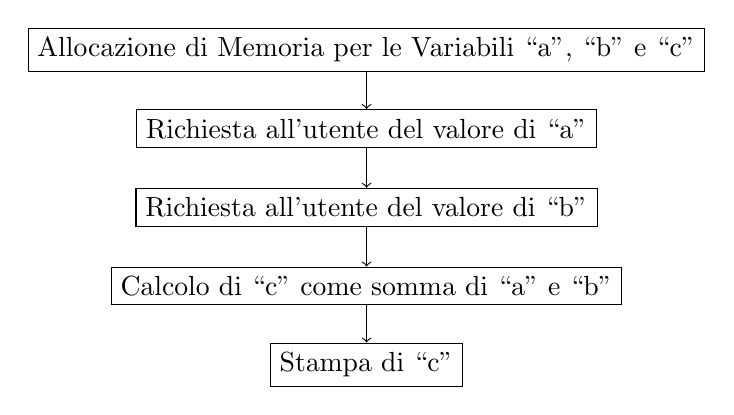
\begin{tikzpicture}

        % Vertices
        \node[rectangle, draw](abcDec){Allocazione di Memoria per le Variabili ``a'', ``b'' e ``c''};
        \node[rectangle, draw](a)[below of = abcDec]{Richiesta all'utente del valore di ``a''};
        \node[rectangle, draw](b)[below of = a]{Richiesta all'utente del valore di ``b''};
        \node[rectangle, draw](cCalc)[below of = b]{Calcolo di ``c'' come somma di ``a'' e ``b''};
        \node[rectangle, draw](c)[below of = cCalc]{Stampa di ``c''};
        % Edges
        \draw[->](abcDec.south) -- (a.north);
        \draw[->](a.south) -- (b.north);
        \draw[->](b.south) -- (cCalc.north);
        \draw[->](cCalc.south) -- (c.north);

    \end{tikzpicture}
    \caption{Grafo delle Precedenze di un Processo Sequenziale.}
    \label{fig.GrafoPrecedenzeOrdTotale}
\end{figure}